\chapter{Propuesta}\label{ch:proposal}

En el presente capítulo se aborda el diseño teórico-computacional de la solución propuesta para satisfacer la 
carencia de un repositorio de imágenes dermatoscópicas unificado dentro del ecosistema DermaUH, cuya 
necesidad fue fundamentada en el Capítulo~\ref{ch:estado-del-arte}. Se expone 
el sustento lógico que rige la construcción de la base de datos, detallando los requerimientos que guiaron 
el desarrollo del sistema. Posteriormente, se presenta la estructuración arquitectónica, los flujogramas 
que describen el recorrido y transformación de la información clínica, y finalmente, el esquema relacional 
de la base de datos diseñada, evidenciando cómo se garantizan las exigencias de flexibilidad y 
escalabilidad para la investigación biomédica y la práctica clínica en Cuba.

La propuesta de la Base de Imágenes de DermaUH surge de la necesidad de mitigar las deficiencias de los sistemas
estudiados en el capítulo anterior y consolidar la información clínica y dermatoscópica recopilada en un 
entorno altamente seguro, estructurado y adaptable. A diferencia de las 
aproximaciones de almacenamiento genérico, la gestión de datos de la salud exige un enfoque centrado en 
la integridad referencial, la trazabilidad del dato médico, el cumplimiento del consentimiento informado 
y la capacidad de realizar estudios epidemiológicos complejos de forma eficiente. 

El modelo concebido adopta el principio de separación de responsabilidades a nivel de arquitectura, 
centralizando las reglas de negocio y validación clínica en una capa de interfaz de programación de 
aplicaciones (API)\footnote{API: conjunto de reglas o protocolos que permite que las aplicaciones de 
software se comuniquen entre sí para intercambiar datos, características y funcionalidades.} 
que puede ser consumida independientemente por aplicaciones móviles y plataformas 
web, posibilitando una integración multimodal.

La aplicación propuesta constituye una base de datos institucional de imágenes dermatoscópicas, diseñada 
para capturar, organizar, consultar y exportar información clínica asociada a lesiones cutáneas. Su 
objetivo es ofrecer un repositorio unificado que facilite la investigación, la docencia y el soporte 
asistencial en el ecosistema DermaUH mediante flujos seguros de carga, clasificación y descarga de datos.

El sistema contempla perfiles de usuarios heterogéneos, desde usuarios comunes o visitantes que acceden 
a material público, hasta especialistas que contribuyen casos clínicos y administradores encargados de 
supervisar la calidad y la visibilidad de los registros. Este enfoque permite que cualquier tipo de 
usuario autorizado interactúe con la plataforma en función de su rol y necesidades de trabajo.

\section{Requerimientos del Sistema}
Para guiar el proceso de desarrollo de \textit{software} con rigor metodológico, se definieron los requerimientos 
del sistema en tres categorías principales: funcionales, no funcionales y de entorno.

\subsection{Requerimientos Funcionales}
Los requerimientos funcionales especifican los comportamientos y servicios exactos que el sistema debe 
proveer a los distintos actores:

\begin{itemize}
    \item \textbf{Gestión de Imágenes Dermatológicas}: El sistema debe permitir la carga de imágenes clínicas y dermatoscópicas, extrayendo y validando rigurosamente los 
    metadatos asociados.
    \item \textbf{Gestión de Metadatos Clínicos}: El sistema debe soportar un esquema de metadatos 
    exhaustivo para cada lesión, abarcando datos demográficos (edad, sexo biológico, color de piel, fototipo), 
    antecedentes (historial personal y familiar de melanoma, exposición solar), información patológica e 
    institucional.
    \item \textbf{Control de Acceso y Visibilidad}: Debe ser posible clasificar las imágenes como públicas 
    o privadas. Las imágenes privadas estarán restringidas a usuarios con roles administrativos.
    \item \textbf{Explotación Analítica y Estadística}: Se requiere que el sistema agrupe, filtre y tabule 
    la información para generar visualizaciones y resúmenes (por ejemplo, distribución demográfica, 
    distribución espacial del melanoma en un mapa corporal).
    \item \textbf{Descarga Masiva}: Debe habilitarse un mecanismo para la descarga de galerías de imágenes 
    seleccionadas en formato comprimido (ZIP), junto con los datos tabulares correspondientes normalizados 
    en archivos CSV (\textit{Comma Separated Values}).
\end{itemize}

\subsection{Requerimientos No Funcionales}
\subsubsection{Requerimientos de Seguridad}

\begin{itemize}
    \item \textbf{Autenticación Robusta}: Implementación de \textit{tokens} de acceso (JWT)~\cite{rfc7519_jwt} y protección de las 
    rutas del API, denegando el acceso a recursos privados si el actor no posee el nivel de autorización 
    requerido~\cite{owasp_secure_default}.
    \item \textbf{Protección de Puntos de Entrada}: Validación estricta a nivel de infraestructura para 
    evitar manipulación de parámetros de negocio a través de validadores robustos.
    \item \textbf{Gestión de Datos Sensibles}: El esquema de identidad debe almacenar las credenciales 
    mediante funciones de hash criptográficas seguras, acoplado al marco de trabajo de identidad nativo 
    de la tecnología de desarrollo.
\end{itemize}

\subsubsection{Requerimientos de Usabilidad}
\begin{itemize}
    \item \textbf{Interfaz Intuitiva y Responsiva}: La interfaz web debe adaptarse fluidamente a las 
    diferentes dimensiones de pantalla y proporcionar una navegación lógica para minimizar la curva 
    de aprendizaje del personal médico.
\end{itemize}

\subsubsection{Requerimientos de Almacenamiento}
\begin{itemize}
    \item \textbf{Persistencia Híbrida}: La arquitectura debe separar lógicamente el almacenamiento de 
    metadatos estructurados (en bases relacionales) del almacenamiento de los archivos binarios, 
    garantizando el rendimiento ante grandes volúmenes de casos clínicos.
\end{itemize}


\subsection{Requerimientos de Entorno}
Para su despliegue y operatividad, la plataforma define como requisitos técnicos y tecnológicos base:
\begin{itemize}
    \item \textbf{Entorno de Ejecución}: \textit{Runtime} multiplataforma compatible con distribuciones 
    de código abierto basadas en Linux (requisito mandatorio para la soberanía tecnológica en los 
    servidores locales). El sistema se basará en la plataforma SDK de .NET versión 10.0.
    \item \textbf{Motor de Bases de Datos}: Un Sistema Gestor de Base de Datos (SGBD) relacional robusto con características avanzadas 
    y alto rendimiento, estableciéndose como objetivo PostgreSQL.
    \item \textbf{Servicios Externos}: Un servidor de Protocolo Simple de Transferencia de Correo (SMTP) para la emisión de notificaciones automatizadas y 
    flujos de restablecimiento de cuenta.
\end{itemize}

\section{Estructuración del Diseño Teórico-Computacional}

\subsection{Arquitectura del Sistema}
Para dar cumplimiento a los requerimientos y maximizar la escalabilidad, el modelo arquitectónico 
implementado adopta un paradigma de \textbf{arquitectura por capas} acoplado al patrón \textbf{cliente-servidor} \cite{client_server}.

\begin{figure}[htbp]
    \centering
    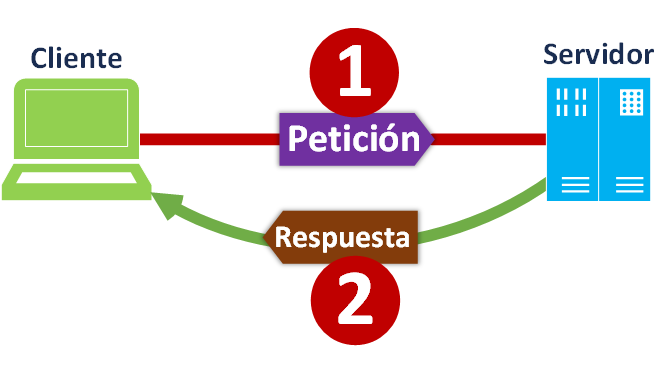
\includegraphics[width=0.85\textwidth]{Graphics/Cliente-Servidor.png}
    \caption{Ilustración del patrón cliente-servidor.}
    \label{fig:cliente_servidor}
\end{figure}

En el patrón cliente-servidor, la responsabilidad se divide entre un cliente que inicia la comunicación y 
un servidor que centraliza el procesamiento y la provisión de recursos. El cliente representa cualquier 
dispositivo o aplicación que consume servicios (por ejemplo, una aplicación web), mientras que el servidor 
expone operaciones y coordina el acceso a datos y reglas de negocio. Este modelo favorece la separación de 
responsabilidades, el control de acceso, la escalabilidad horizontal y la administración centralizada de 
los recursos \cite{client_server}.

El esquema de funcionamiento básico es el siguiente:
\begin{enumerate}
    \item El cliente solicita una información o servicio al servidor.
    \item El servidor recibe la petición.
    \item El servidor procesa la solicitud con las reglas de negocio y el acceso a datos correspondiente.
    \item El servidor envía el resultado al cliente.
    \item El cliente recibe la respuesta y la presenta o procesa en su interfaz.
\end{enumerate}


La estructura del \textit{backend}\footnote{Backend: capa del servidor responsable de la lógica de negocio, persistencia y exposición de servicios.} se divide lógicamente en~\cite{martin_clean_architecture}:
\begin{enumerate}
    \item \textbf{Capa de Dominio (\textit{Domain})}: Constituye el núcleo del sistema, encapsulando el 
    modelo de información clínica (entidades fundamentales) y enumeraciones médicas, operando libre de 
    dependencias a marcos de trabajo externos.
    \item \textbf{Capa de Aplicación (\textit{Application})}: Contiene la lógica de negocio, aplicando 
    validaciones clínicas a través de reglas condicionales estandarizadas antes de interactuar 
    con el dominio de la información.
    \item \textbf{Capa de Infraestructura (\textit{Infrastructure})}: Centraliza el almacenamiento a 
    disco y bases de datos, utilizando tecnología de mapeo objeto-relacional\footnote{ORM (\textit{Object-Relational Mapping}): técnica de programación que permite interactuar con una base de datos relacional utilizando objetos del lenguaje de programación.} (ORM) para generar 
    migraciones eficientes hacia PostgreSQL~\cite{ef_core_docs,postgresql_docs}.
    \item \textbf{Capa de Presentación y Puntos de Acceso (\textit{WebApi})}: Expone los servicios de la 
    plataforma a los clientes mediante terminales controladas (\textit{endpoints}), documentados con el 
    estándar OpenAPI\footnote{OpenAPI: estándar reconocido a nivel mundial para describir, producir, consumir 
    y visualizar APIs HTTP RESTful.}~\cite{openapi_spec}.
\end{enumerate}

\begin{figure}[H]
    \centering
    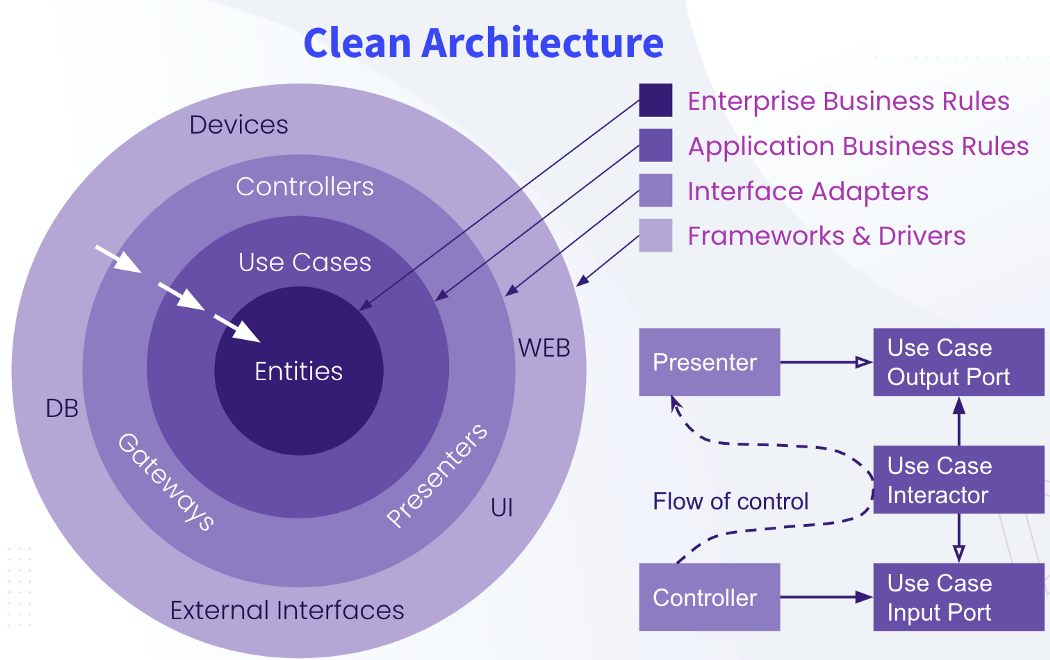
\includegraphics[width=0.85\textwidth]{Graphics/clean-architecture.png}
    \caption{Patrón arquitectónico por capas.}
    \label{fig:clean_architecture}
\end{figure}

Por su parte, la interfaz clínica se implementa como una aplicación cliente interactiva de 
tipo \textit{server-side}, desplegada en el servidor mediante \textit{Blazor Server}~\cite{blazor_docs}. Esta capa 
de \textit{frontend}\footnote{Frontend: capa de interfaz que presenta la información y permite la 
interacción del usuario con el sistema.} orquesta la presentación, la navegación y la captura de entradas, 
consumiendo de forma controlada los servicios expuestos por la API, con intercambio eficiente de estados 
y baja latencia percibida.

\subsection{Casos de Uso del Sistema}
Los casos de uso del sistema se agrupan en módulos funcionales. Para cada caso se especifica el actor autorizado, una descripción del comportamiento y, cuando corresponde, el flujo de operaciones que sigue el sistema.

\subsubsection{Módulo de Autenticación y Gestión de Cuenta}

\paragraph{CU-01: Registrar Usuario.}
\begin{description}
    \item[Actor:] Cualquier persona (anónimo).
    \item[Descripción:] Un nuevo usuario se registra proporcionando nombre, apellido, correo electrónico y contraseña. El sistema envía un correo de confirmación y la cuenta permanece inactiva hasta ser aprobada por un administrador.
    \item[Flujo:]~
    \begin{enumerate}
        \item El usuario envía los datos de registro (nombre, apellido, email, contraseña).
        \item El sistema verifica la inexistencia de duplicados y crea la cuenta.
        \item Se genera un \textit{token} de confirmación de correo electrónico.
        \item Se envía un correo de confirmación al usuario.
        \item Se notifica al administrador sobre el nuevo registro pendiente.
    \end{enumerate}
    \item[Postcondición:] Usuario creado con cuenta inactiva y correo sin confirmar.
\end{description}

\paragraph{CU-02: Confirmar Email.}
\begin{description}
    \item[Actor:] Usuario registrado (anónimo).
    \item[Descripción:] El usuario accede al enlace recibido por correo. El sistema valida el \textit{token} y marca la dirección de correo electrónico como confirmada.
    \item[Flujo:]~
    \begin{enumerate}
        \item El usuario envía el identificador de usuario y el \textit{token} de confirmación.
        \item El sistema valida el \textit{token} con el marco de identidad.
        \item El estado de confirmación del correo se establece como verdadero.
    \end{enumerate}
\end{description}

\paragraph{CU-03: Iniciar Sesión (Email/Contraseña).}
\begin{description}
    \item[Actor:] Usuario registrado y activo.
    \item[Descripción:] El usuario se autentica con su correo electrónico y contraseña. El sistema devuelve un \textit{token} JWT con los roles asignados.
    \item[Flujo:]~
    \begin{enumerate}
        \item El usuario envía sus credenciales (email, contraseña).
        \item El sistema valida las credenciales.
        \item Se obtienen los roles del usuario.
        \item El servicio JWT genera el \textit{token} con los \textit{claims} y roles correspondientes.
        \item Se retorna el \textit{token}, el identificador de usuario y sus roles.
    \end{enumerate}
\end{description}

\paragraph{CU-04: Iniciar Sesión con Google OAuth2.}
\begin{description}
    \item[Actor:] Cualquier persona (anónimo).
    \item[Descripción:] El usuario se autentica usando su cuenta de Google. El sistema valida el \textit{token} de identidad de Google y genera un JWT propio del sistema.
    \item[Flujo:]~
    \begin{enumerate}
        \item El usuario envía el \textit{token} de identidad de Google.
        \item El sistema valida el \textit{token} con la biblioteca de autenticación de Google.
        \item Si el usuario no existe en el sistema, se crea automáticamente.
        \item Se genera el JWT del sistema.
    \end{enumerate}
\end{description}

\paragraph{CU-05: Recuperar Contraseña.}
\begin{description}
    \item[Actor:] Usuario registrado (anónimo).
    \item[Descripción:] El usuario solicita un enlace de restablecimiento de contraseña. El sistema envía un correo con el \textit{token} de restablecimiento.
    \item[Flujo:]~
    \begin{enumerate}
        \item El usuario envía su dirección de correo electrónico.
        \item El sistema genera un \textit{token} de restablecimiento.
        \item Se envía un correo con el enlace de restablecimiento.
        \item La respuesta siempre es satisfactoria (por seguridad, no se revela si el correo existe).
    \end{enumerate}
\end{description}

\paragraph{CU-06: Restablecer Contraseña.}
\begin{description}
    \item[Actor:] Usuario registrado (anónimo con \textit{token}).
    \item[Descripción:] El usuario establece una nueva contraseña utilizando el \textit{token} recibido por correo electrónico.
\end{description}

\paragraph{CU-07: Ver Perfil de Usuario.}
\begin{description}
    \item[Actor:] Usuario autenticado (cualquier rol).
    \item[Descripción:] El usuario consulta su información de perfil, incluyendo nombre, correo electrónico, roles asignados y estado de autorización de descarga.
\end{description}

\paragraph{CU-08: Actualizar Perfil de Usuario.}
\begin{description}
    \item[Actor:] Usuario autenticado (cualquier rol).
    \item[Descripción:] El usuario actualiza su nombre, apellido u otros datos de perfil.
\end{description}

\paragraph{CU-09: Cambiar Contraseña.}
\begin{description}
    \item[Actor:] Usuario autenticado (cualquier rol).
    \item[Descripción:] El usuario cambia su contraseña actual por una nueva, proporcionando la contraseña vigente para verificación.
\end{description}

\subsubsection{Módulo de Gestión de Imágenes}

\paragraph{CU-10: Consultar Galería de Imágenes.}
\begin{description}
    \item[Actor:] Anónimo / cualquier usuario autenticado.
    \item[Descripción:] Consulta paginada de imágenes públicas con filtros múltiples. Solo devuelve imágenes con visibilidad pública.
    \item[Filtros disponibles:] tipo de imagen, categoría diagnóstica, tipo de lesión, fototipo (Fitzpatrick), sexo, sitio anatómico general, método de confirmación diagnóstica, búsqueda textual por diagnóstico.
\end{description}

\paragraph{CU-11: Ver Detalle de Imagen.}
\begin{description}
    \item[Actor:] Anónimo / cualquier usuario autenticado.
    \item[Descripción:] Obtiene los metadatos completos de una imagen. Se aplica control de acceso: las imágenes privadas solo son visibles para administradores.
\end{description}

\paragraph{CU-12: Previsualizar Imagen.}
\begin{description}
    \item[Actor:] Anónimo / cualquier usuario autenticado.
    \item[Descripción:] Transmite el archivo físico de la imagen al cliente. Verifica permisos de acceso antes de servir el archivo y soporta peticiones de rango para \textit{streaming} eficiente.
\end{description}

\paragraph{CU-13: Subir Nueva Imagen con Metadatos Clínicos.}
\begin{description}
    \item[Actor:] Administrador, Colaborador.
    \item[Descripción:] Sube una imagen dermatológica junto con sus metadatos clínicos. El sistema almacena el archivo en disco y persiste los metadatos en la base de datos.
    \item[Flujo:]~
    \begin{enumerate}
        \item El colaborador envía el archivo de imagen junto con los metadatos clínicos.
        \item El gestor de carga almacena el archivo en el directorio raíz configurado.
        \item Se aplican las reglas de validación clínica.
        \item El sistema persiste la entidad con un identificador público generado automáticamente.
        \item Se retorna la respuesta con el registro creado.
    \end{enumerate}
    \item[Validaciones obligatorias:] edad aproximada, sexo, sitio anatómico general, diagnóstico, exposición solar.
    \item[Validaciones condicionales:]~
    \begin{itemize}
        \item Tipo de lesión, solo si la categoría diagnóstica es maligna.
        \item Tipo dermoscópico, solo si el tipo de imagen es dermoscópica.
        \item Campos histológicos de melanoma, solo si el tipo de lesión es melanoma.
    \end{itemize}
\end{description}

\paragraph{CU-14: Eliminar Imagen.}
\begin{description}
    \item[Actor:] Administrador.
    \item[Descripción:] Realiza un borrado lógico de la imagen. El registro no se elimina físicamente de la base de datos ni del sistema de archivos.
\end{description}

\paragraph{CU-15: Descargar Imágenes Seleccionadas (ZIP).}
\begin{description}
    \item[Actor:] Usuario autenticado con autorización de descarga.
    \item[Descripción:] Genera y descarga un archivo ZIP con las imágenes seleccionadas y/o sus metadatos en formato CSV.
    \item[Modos de descarga:] imágenes y metadatos, solo metadatos, solo imágenes.
    \item[Flujo:]~
    \begin{enumerate}
        \item El usuario envía la lista de identificadores de imágenes y el modo de descarga.
        \item Se verifica el acceso a cada imagen.
        \item Se construye el archivo ZIP con las imágenes y/o el archivo CSV de metadatos.
        \item Si faltan archivos físicos, se incluye un registro de errores en el ZIP.
    \end{enumerate}
\end{description}

\paragraph{CU-16: Descargar Todas las Imágenes Filtradas (ZIP).}
\begin{description}
    \item[Actor:] Usuario autenticado con autorización de descarga.
    \item[Descripción:] Genera un archivo ZIP con todas las imágenes públicas que coincidan con los filtros aplicados. Acepta los mismos filtros que la galería.
\end{description}

\subsubsection{Módulo de Gestión de Usuarios}

\paragraph{CU-18: Listar Todos los Usuarios.}
\begin{description}
    \item[Actor:] Administrador.
    \item[Descripción:] Obtiene la lista paginada de todos los usuarios del sistema con sus roles asignados.
\end{description}

\paragraph{CU-19: Ver Detalle de Usuario.}
\begin{description}
    \item[Actor:] Administrador.
    \item[Descripción:] Obtiene la información completa de un usuario específico, incluyendo sus roles.
\end{description}

\paragraph{CU-20: Crear Usuario.}
\begin{description}
    \item[Actor:] Administrador.
    \item[Descripción:] El administrador crea un nuevo usuario directamente desde el panel de administración, sin necesidad de que el usuario se registre por sí mismo.
\end{description}

\paragraph{CU-21: Asignar Rol a Usuario.}
\begin{description}
    \item[Actor:] Administrador.
    \item[Descripción:] Asigna un rol (\textit{Admin}, \textit{Viewer}, \textit{Contributor}) a un usuario específico.
\end{description}

\paragraph{CU-22: Remover Rol de Usuario.}
\begin{description}
    \item[Actor:] Administrador.
    \item[Descripción:] Elimina un rol previamente asignado a un usuario.
\end{description}

\paragraph{CU-23: Activar/Desactivar Usuario.}
\begin{description}
    \item[Actor:] Administrador.
    \item[Descripción:] Cambia el estado de activación de un usuario. Un usuario inactivo no puede iniciar sesión.
\end{description}

\paragraph{CU-24: Eliminar Usuario.}
\begin{description}
    \item[Actor:] Administrador.
    \item[Descripción:] Realiza un borrado lógico del usuario para salvaguardar la integridad referencial.
\end{description}

\paragraph{CU-25: Aprobar Registro de Usuario.}
\begin{description}
    \item[Actor:] Administrador.
    \item[Descripción:] Aprueba el registro pendiente de un usuario, activando su cuenta. Se envía una notificación por correo electrónico al usuario aprobado.
    \item[Flujo:]~
    \begin{enumerate}
        \item El administrador consulta la lista de registros pendientes.
        \item El administrador aprueba un usuario específico.
        \item El sistema establece la cuenta como activa.
        \item Se envía un correo de notificación de aprobación al usuario.
    \end{enumerate}
\end{description}

\paragraph{CU-26: Rechazar Registro de Usuario.}
\begin{description}
    \item[Actor:] Administrador.
    \item[Descripción:] Rechaza el registro de un usuario y elimina la cuenta. Se envía un correo de rechazo al usuario.
\end{description}

\subsubsection{Módulo de Solicitudes de Descarga}

\paragraph{CU-27: Solicitar Autorización de Descarga.}
\begin{description}
    \item[Actor:] Usuario autenticado (cualquier rol).
    \item[Descripción:] El usuario solicita permiso para descargar imágenes de forma masiva. Debe proporcionar una justificación y su institución.
    \item[Flujo:]~
    \begin{enumerate}
        \item El usuario envía la justificación y el nombre de su institución.
        \item El sistema crea la solicitud con estado pendiente.
        \item Se notifica a todos los administradores activos por correo electrónico.
    \end{enumerate}
\end{description}

\paragraph{CU-28: Ver Solicitudes de Descarga Pendientes.}
\begin{description}
    \item[Actor:] Administrador.
    \item[Descripción:] Obtiene la lista paginada de solicitudes de descarga con estado pendiente para la cola de revisión del administrador.
\end{description}

\paragraph{CU-29: Revisar Solicitud de Descarga.}
\begin{description}
    \item[Actor:] Administrador.
    \item[Descripción:] El administrador aprueba o rechaza una solicitud de descarga.
    \item[Flujo (aprobación):]~
    \begin{enumerate}
        \item El administrador aprueba la solicitud.
        \item El sistema actualiza el estado de la solicitud.
        \item Se habilita la autorización de descarga para el usuario.
        \item Se envía un correo de aprobación al usuario.
    \end{enumerate}
    \item[Flujo (rechazo):]~
    \begin{enumerate}
        \item El administrador rechaza la solicitud.
        \item La autorización de descarga del usuario permanece deshabilitada.
        \item Se envía un correo de rechazo al usuario.
    \end{enumerate}
\end{description}

\paragraph{CU-30: Ver Mis Solicitudes de Descarga.}
\begin{description}
    \item[Actor:] Usuario autenticado (cualquier rol).
    \item[Descripción:] El usuario consulta el historial y estado de sus propias solicitudes de descarga.
\end{description}

\paragraph{CU-31: Verificar Estado de Autorización.}
\begin{description}
    \item[Actor:] Usuario autenticado (cualquier rol).
    \item[Descripción:] Verifica si el usuario actual tiene autorización activa para descargar imágenes de forma masiva.
\end{description}

\subsubsection{Módulo de Estadísticas y Analítica}

\paragraph{CU-32: Consultar Estadísticas Generales.}
\begin{description}
    \item[Actor:] Anónimo / administrador (con datos extendidos).
    \item[Descripción:] Retorna métricas agregadas para el cuadro de mando analítico. Los administradores reciben estadísticas que incluyen imágenes privadas; los usuarios anónimos solo acceden a datos públicos.
    \item[Datos incluidos:] total de imágenes, conteo por institución, distribución por categoría diagnóstica, distribución por sexo, distribución por sitio anatómico, tabulaciones cruzadas y completitud de datos.
\end{description}

\subsubsection{Módulo de Instituciones}

\paragraph{CU-33: Listar Instituciones Contribuyentes.}
\begin{description}
    \item[Actor:] Usuario autenticado (cualquier rol).
    \item[Descripción:] Retorna el directorio de instituciones médicas que han contribuido imágenes a la base de datos. Los datos se derivan de los metadatos de las imágenes, no de una tabla separada.
\end{description}

\subsubsection{Módulo de Metadatos}

\paragraph{CU-34: Consultar Diccionario de Metadatos.}
\begin{description}
    \item[Actor:] Anónimo / cualquier usuario.
    \item[Descripción:] Retorna la definición completa de los campos de metadatos clínicos, incluyendo nombre, tipo de dato y descripción de cada campo.
\end{description}

\paragraph{CU-35: Descargar Diccionario de Metadatos en CSV.}
\begin{description}
    \item[Actor:] Anónimo / cualquier usuario.
    \item[Descripción:] Genera y descarga un archivo CSV con la definición de todos los campos de metadatos del sistema.
\end{description}

\subsection{Flujogramas de Información}

El ciclo de la información sigue procesos formales para asegurar la validez del \textit{corpus}:

\textbf{Subida e Integración de Imágenes:}
El contribuidor inicia la transferencia de una imagen y sus metadatos asociados. El componente de API 
recibe la estructura segmentada (\textit{multipart/form-data}) y somete los campos textuales a 
verificaciones médicas transversales (por ejemplo, asegurando que métricas histológicas de un 
melanoma no sean asociadas erróneamente a carcinomas inespecíficos). Una vez garantizada su 
coherencia analítica, el gestor de archivos ubica de manera definitiva el binario de imagen 
en un entorno aislado, previniendo colisiones lógicas, mientras delega a la capa infraestructural 
el registro atómico y definitivo de la entidad principal.

\textbf{Descarga y Exportación Masiva:}
Al recibir una solicitud del usuario que agrupa criterios variables mediante flujos de filtros, el 
controlador identifica primero el perfil de visibilidad del solicitante asegurando que no transgreda la 
privacidad de registros privados. Posteriormente genera dinámicamente un canal de almacenamiento 
transitorio (\textit{stream}), donde procede a consolidar todos los ficheros de las imágenes. 
Simultáneamente el catalogador de metadatos del proyecto compila y codifica todos los atributos 
relacionales en un fichero textual de variables separadas por comas (CSV), ensamblando un archivo 
ZIP.

\subsection{Esquema de Base de Datos}
La base de datos seleccionada para el sistema es PostgreSQL~\cite{postgresql_docs}, gestionada mediante el mapeador objeto-relacional Entity Framework Core~\cite{ef_core_docs}. El esquema diseñado combina tablas propias del dominio clínico con el esquema estándar de identidad de ASP.NET Core Identity~\cite{aspnet_identity} para el control de acceso.

\subsubsection{Tabla \texttt{Images} (Entidad \texttt{DermaImg})}
Constituye la tabla principal del sistema. Almacena las imágenes dermatológicas junto a la totalidad de sus metadatos clínicos e institucionales.

\paragraph{Campos de identificación y control.}~

\begin{longtable}{|p{3.5cm}|p{4cm}|p{7cm}|}
\hline
\textbf{Campo} & \textbf{Tipo SQL} & \textbf{Descripción} \\
\hline
\endfirsthead
\hline
\textbf{Campo} & \textbf{Tipo SQL} & \textbf{Descripción} \\
\hline
\endhead
\texttt{Id} & \texttt{uuid} PK & Identificador interno único (GUID). \\
\hline
\texttt{PublicId} & \texttt{varchar(30)} UNIQUE NOT NULL & Identificador público legible (ej. DERM\_0000001). \\
\hline
\texttt{FileName} & \texttt{varchar(500)} NOT NULL & Nombre original del archivo subido. \\
\hline
\texttt{FilePath} & \texttt{varchar(1000)} NOT NULL & Ruta absoluta del archivo en el servidor. \\
\hline
\texttt{ContentType} & \texttt{varchar(100)} NOT NULL & Tipo MIME del archivo (ej. \texttt{image/jpeg}). \\
\hline
\texttt{FileSize} & \texttt{bigint} NOT NULL & Tamaño del archivo en bytes. \\
\hline
\texttt{IsPublic} & \texttt{boolean} NOT NULL & Si es verdadero, visible para usuarios anónimos. \\
\hline
\texttt{IsDeleted} & \texttt{boolean} NOT NULL & Eliminación lógica: si es verdadero, excluido de consultas. \\
\hline
\texttt{CreatedAt} & \texttt{timestamp with time zone} & Fecha de creación del registro. \\
\hline
\texttt{UpdatedAt} & \texttt{timestamp with time zone} NULL & Fecha de última actualización. \\
\hline
\texttt{ContributorId} & \texttt{uuid} NOT NULL & Identificador del usuario externo que subió la imagen. \\
\hline
\end{longtable}

\paragraph{Campos de adquisición técnica.}~

\begin{longtable}{|p{3.5cm}|p{4cm}|p{7cm}|}
\hline
\textbf{Campo} & \textbf{Tipo SQL} & \textbf{Descripción} \\
\hline
\endfirsthead
\hline
\textbf{Campo} & \textbf{Tipo SQL} & \textbf{Descripción} \\
\hline
\endhead
\texttt{ImageType} & \texttt{varchar(50)} NULL & Modalidad de captura: \textit{Dermoscopic}, \textit{ClinicalOverview}, \textit{ClinicalCloseUp}, entre otras. \\
\hline
\texttt{ImageManipulation} & \texttt{varchar(50)} NULL & Fidelidad respecto a la captura original. \\
\hline
\texttt{DermoscopicType} & \texttt{varchar(50)} NULL & Modalidad dermoscópica (solo si \texttt{ImageType} = \textit{Dermoscopic}). \\
\hline
\end{longtable}

\paragraph{Campos demográficos del paciente.}~

\begin{longtable}{|p{3.5cm}|p{4cm}|p{7cm}|}
\hline
\textbf{Campo} & \textbf{Tipo SQL} & \textbf{Descripción} \\
\hline
\endfirsthead
\hline
\textbf{Campo} & \textbf{Tipo SQL} & \textbf{Descripción} \\
\hline
\endhead
\texttt{AgeApprox} & \texttt{integer} NULL & Edad aproximada del paciente (0--120). \\
\hline
\texttt{Sex} & \texttt{varchar(20)} NULL & Sexo biológico: \textit{Male}, \textit{Female}. \\
\hline
\texttt{SkinColor} & \texttt{varchar(30)} NULL & Clasificación de color de piel. \\
\hline
\texttt{FotoType} & \texttt{varchar(50)} NULL & Fototipo de Fitzpatrick. \\
\hline
\texttt{PersonalHistory} & \texttt{varchar(1000)} NULL & Antecedentes personales del paciente. \\
\hline
\texttt{PersonalHxMm} & \texttt{boolean} NULL & Antecedente personal de melanoma. \\
\hline
\texttt{FamilyHxMm} & \texttt{boolean} NULL & Antecedente familiar de melanoma. \\
\hline
\texttt{SunExposure} & \texttt{boolean} NULL & Exposición solar reportada. \\
\hline
\texttt{Provincia} & \texttt{varchar(50)} NULL & Provincia de procedencia del paciente. \\
\hline


\end{longtable}

\paragraph{Campos clínicos de la lesión.}~

\begin{longtable}{|p{3.5cm}|p{4cm}|p{7cm}|}
\hline
\textbf{Campo} & \textbf{Tipo SQL} & \textbf{Descripción} \\
\hline
\endfirsthead
\hline
\textbf{Campo} & \textbf{Tipo SQL} & \textbf{Descripción} \\
\hline
\endhead
\texttt{AnatomSite\-General} & \texttt{varchar(50)} NULL & Localización anatómica general: \textit{HeadNeck}, \textit{UpperExtremity}, \textit{LowerExtremity}, \textit{AnteriorTorso}, \textit{PosteriorTorso}, \textit{PalmsSoles}, \textit{OralGenital}. \\
\hline
\texttt{AnatomSite\-Special} & \texttt{varchar(50)} NULL & Sitio anatómico especial (acral, uña, etc.). \\
\hline
\texttt{ClinSizeLong\-DiamMm} & \texttt{double precision} NULL & Diámetro mayor de la lesión en mm. \\
\hline
\end{longtable}

\paragraph{Campos diagnósticos.}~

\begin{longtable}{|p{3.5cm}|p{4cm}|p{7cm}|}
\hline
\textbf{Campo} & \textbf{Tipo SQL} & \textbf{Descripción} \\
\hline
\endfirsthead
\hline
\textbf{Campo} & \textbf{Tipo SQL} & \textbf{Descripción} \\
\hline
\endhead
\texttt{Diagnosis} & \texttt{varchar(500)} NULL & Diagnóstico textual del contribuidor. \\
\hline
\texttt{Histopathological\-Diagnosis} & \texttt{varchar(500)} NULL & Diagnóstico histopatológico. \\
\hline
\texttt{Diagnosis\-Category} & \texttt{varchar(50)} NULL & Categoría de malignidad: \textit{Benign}, \textit{Indeterminate}, \textit{Malignant}. \\
\hline
\texttt{InjuryType} & \texttt{varchar(50)} NULL & Tipo de lesión maligna: \textit{Melanoma}, \textit{BasalCellCarcinoma}, \textit{SquamousCellCarcinoma}, \textit{Others} (solo si la categoría es maligna). \\
\hline
\texttt{Diagnosis\-ConfirmType} & \texttt{varchar(100)} NULL & Método de confirmación diagnóstica: \textit{Histopathology}, \textit{ClinicalFollowUp}, etc. \\
\hline
\end{longtable}

\paragraph{Campos histológicos (específicos de melanoma).}~

\begin{longtable}{|p{3.5cm}|p{4cm}|p{7cm}|}
\hline
\textbf{Campo} & \textbf{Tipo SQL} & \textbf{Descripción} \\
\hline
\endfirsthead
\hline
\textbf{Campo} & \textbf{Tipo SQL} & \textbf{Descripción} \\
\hline
\endhead
\texttt{MelThickMm} & \texttt{double precision} NULL & Profundidad de Breslow en mm (solo si \texttt{InjuryType} = \textit{Melanoma}). \\
\hline
\texttt{MelMitoticIndex} & \texttt{varchar(50)} NULL & Índice mitótico del melanoma. \\
\hline
\texttt{MelUlcer} & \texttt{boolean} NULL & Presencia de ulceración histopatológica. \\
\hline
\end{longtable}

\paragraph{Campos de notas y consentimiento.}~

\begin{longtable}{|p{3.5cm}|p{4cm}|p{7cm}|}
\hline
\textbf{Campo} & \textbf{Tipo SQL} & \textbf{Descripción} \\
\hline
\endfirsthead
\hline
\textbf{Campo} & \textbf{Tipo SQL} & \textbf{Descripción} \\
\hline
\endhead
\texttt{ClinicalNotes} & \texttt{varchar(2000)} NULL & Notas clínicas en texto libre. \\
\hline
\texttt{Dermoscopic\-Comments} & \texttt{varchar(2000)} NULL & Observaciones dermoscópicas del especialista. \\
\hline
\texttt{InformedConsent} & \texttt{boolean} NULL & Indica si se obtuvo consentimiento informado. \\
\hline
\texttt{InformedConsent\-Date} & \texttt{timestamp with time zone} NULL & Fecha de firma del consentimiento. \\
\hline
\texttt{InformedConsent\-Text} & \texttt{varchar(4000)} NULL & Texto o referencia del documento de consentimiento. \\
\hline
\end{longtable}

\paragraph{Campos de metadatos institucionales.}~

\begin{longtable}{|p{3.5cm}|p{4cm}|p{7cm}|}
\hline
\textbf{Campo} & \textbf{Tipo SQL} & \textbf{Descripción} \\
\hline
\endfirsthead
\hline
\textbf{Campo} & \textbf{Tipo SQL} & \textbf{Descripción} \\
\hline
\endhead
\texttt{InstitutionName} & \texttt{varchar(200)} NULL & Nombre de la institución contribuyente. \\
\hline
\texttt{Institution\-Description} & \texttt{varchar(1000)} NULL & Descripción de la institución. \\
\hline
\texttt{Institution\-Country} & \texttt{varchar(100)} NULL & País de la institución. \\
\hline
\end{longtable}

\subsubsection{Tabla \texttt{Users} (Entidad \texttt{User})}
Extiende el modelo de usuario estándar (\texttt{IdentityUser<Guid>}) de ASP.NET Core Identity con campos de perfil y control de acceso propios del dominio.

\begin{longtable}{|p{3.5cm}|p{4cm}|p{7cm}|}
\hline
\textbf{Campo} & \textbf{Tipo SQL} & \textbf{Descripción} \\
\hline
\endfirsthead
\hline
\textbf{Campo} & \textbf{Tipo SQL} & \textbf{Descripción} \\
\hline
\endhead
\texttt{Id} & \texttt{uuid} PK & Identificador único del usuario. \\
\hline
\texttt{FirstName} & \texttt{varchar(100)} NOT NULL & Nombre del usuario. \\
\hline
\texttt{LastName} & \texttt{varchar(100)} NOT NULL & Apellido del usuario. \\
\hline
\texttt{Email} & \texttt{varchar(256)} NULL & Correo electrónico (único). \\
\hline
\texttt{NormalizedEmail} & \texttt{varchar(256)} NULL & Email normalizado para búsquedas (índice). \\
\hline
\texttt{UserName} & \texttt{varchar(256)} NULL & Nombre de usuario. \\
\hline
\texttt{Normalized\-UserName} & \texttt{varchar(256)} NULL & Nombre de usuario normalizado (índice único). \\
\hline
\texttt{PasswordHash} & \texttt{text} NULL & Hash de la contraseña. \\
\hline
\texttt{EmailConfirmed} & \texttt{boolean} NOT NULL & Si el correo fue confirmado. \\
\hline
\texttt{IsActive} & \texttt{boolean} NOT NULL & Si la cuenta está activa (aprobada por administrador). \\
\hline
\texttt{IsDeleted} & \texttt{boolean} NOT NULL & Eliminación lógica. \\
\hline
\texttt{CreatedAt} & \texttt{timestamp with time zone} & Fecha de registro. \\
\hline
\texttt{UpdatedAt} & \texttt{timestamp with time zone} NULL & Fecha de última actualización. \\
\hline
\texttt{SecurityStamp} & \texttt{text} NULL & Sello de seguridad para invalidar \textit{tokens}. \\
\hline
\texttt{Concurrency\-Stamp} & \texttt{text} NULL & Control de concurrencia optimista. \\
\hline
\texttt{PhoneNumber} & \texttt{text} NULL & Número de teléfono. \\
\hline
\texttt{PhoneNumber\-Confirmed} & \texttt{boolean} NOT NULL & Si el teléfono fue confirmado. \\
\hline
\texttt{TwoFactor\-Enabled} & \texttt{boolean} NOT NULL & Si la autenticación de dos factores está habilitada. \\
\hline
\texttt{LockoutEnd} & \texttt{timestamp with time zone} NULL & Fin del bloqueo de cuenta. \\
\hline
\texttt{LockoutEnabled} & \texttt{boolean} NOT NULL & Si el bloqueo está habilitado. \\
\hline
\texttt{AccessFailed\-Count} & \texttt{integer} NOT NULL & Contador de intentos fallidos de inicio de sesión. \\
\hline
\end{longtable}

\subsubsection{Tabla \texttt{DownloadRequests} (Entidad \texttt{DownloadRequest})}
Gestiona el flujo de trabajo de las autorizaciones para descargas masivas de conjuntos de imágenes.

\begin{longtable}{|p{3.5cm}|p{4cm}|p{7cm}|}
\hline
\textbf{Campo} & \textbf{Tipo SQL} & \textbf{Descripción} \\
\hline
\endfirsthead
\hline
\textbf{Campo} & \textbf{Tipo SQL} & \textbf{Descripción} \\
\hline
\endhead
\texttt{Id} & \texttt{uuid} PK & Identificador único de la solicitud. \\
\hline
\texttt{UserId} & \texttt{uuid} NOT NULL FK $\rightarrow$ \texttt{Users.Id} & Usuario que realizó la solicitud. \\
\hline
\texttt{Reason} & \texttt{varchar(2000)} NOT NULL & Justificación de la solicitud de descarga. \\
\hline
\texttt{Institution} & \texttt{varchar(500)} NOT NULL & Institución del solicitante. \\
\hline
\texttt{Status} & \texttt{varchar(50)} NOT NULL & Estado: \textit{Pending}, \textit{Approved}, \textit{Denied}. \\
\hline
\texttt{ReviewedById} & \texttt{uuid} NULL FK $\rightarrow$ \texttt{Users.Id} & Administrador que revisó la solicitud. \\
\hline
\texttt{ReviewedAt} & \texttt{timestamp with time zone} NULL & Fecha de revisión. \\
\hline
\texttt{CreatedAt} & \texttt{timestamp with time zone} & Fecha de creación. \\
\hline
\texttt{UpdatedAt} & \texttt{timestamp with time zone} NULL & Fecha de última actualización. \\
\hline
\texttt{IsDeleted} & \texttt{boolean} NOT NULL & Eliminación lógica. \\
\hline
\end{longtable}

\subsubsection{Tablas de ASP.NET Core Identity}
El sistema complementa las tablas de dominio con las tablas estándar del marco de identidad:

\begin{longtable}{|p{3cm}|p{11.5cm}|}
\hline
\textbf{Tabla} & \textbf{Descripción} \\
\hline
\endfirsthead
\hline
\textbf{Tabla} & \textbf{Descripción} \\
\hline
\endhead
\texttt{Roles} & Roles del sistema (\textit{Admin}, \textit{Viewer}, \textit{Contributor}). \\
\hline
\texttt{UserRoles} & Tabla pivote N:M entre \texttt{Users} y \texttt{Roles}. \\
\hline
\texttt{UserClaims} & \textit{Claims} adicionales por usuario. \\
\hline
\texttt{UserLogins} & Proveedores de inicio de sesión externos (Google OAuth2). \\
\hline
\texttt{UserTokens} & \textit{Tokens} de confirmación de correo, restablecimiento de contraseña, etc. \\
\hline
\texttt{RoleClaims} & \textit{Claims} asociados a roles. \\
\hline
\end{longtable}


\subsubsection{Patrones de Persistencia}
\begin{itemize}
    \item \textbf{Eliminación lógica (\textit{Soft-Delete}):} Entidades esenciales como imágenes, usuarios y solicitudes implementan el campo \texttt{IsDeleted}, excluyéndose automáticamente de consultas estándar mediante filtros globales.
    \item \textbf{Enumeraciones tipadas:} Las categorías finitas se almacenan como cadenas de texto (\texttt{varchar}) para maximizar la legibilidad directa en el gestor de bases de datos.
    \item \textbf{Identificador público único:} La tabla \texttt{Images} posee un índice único sobre \texttt{PublicId} para garantizar la unicidad del identificador público legible.
\end{itemize}

\section{Valoración del Esquema Propuesto para el Entrenamiento de Modelos de Inteligencia Artificial}

El diseño del esquema de datos presentado en este capítulo no responde únicamente a las necesidades operativas inmediatas de gestión y consulta de imágenes dermatológicas. Su concepción se fundamenta en las deficiencias estructurales identificadas durante el análisis exhaustivo del estado del arte (Capítulo~\ref{ch:estado-del-arte}), y persigue como objetivo estratégico que los datos recopilados constituyan un activo de alto valor para el entrenamiento, la validación y el ajuste fino (\textit{fine-tuning}) de modelos de aprendizaje profundo.

\subsection{Riqueza de Metadatos como Habilitador de la Inteligencia Artificial Multimodal}

El análisis de los repositorios internacionales reveló una tendencia clara en la evolución de la dermatología computacional: la transición desde modelos puramente visuales hacia arquitecturas multimodales que integran la imagen con el contexto clínico del paciente~\cite{pmc_padufes}. El conjunto PAD-UFES-20, con sus 26 variables estructuradas por registro, demostró que la combinación de datos sintomáticos, antecedentes y factores socioeconómicos permite a las redes neuronales emular el razonamiento clínico holístico de un especialista. De manera análoga, el repositorio Derm7pt evidenció que las anotaciones conceptuales granulares habilitan la construcción de modelos de cuello de botella conceptual (\textit{Concept Bottleneck Models}), capaces de justificar sus predicciones mediante una cadena de razonamiento auditable~\cite{arxiv_derm7pt_concept}.

El esquema de la entidad \texttt{DermaImg} de la base de datos propuesta fue diseñado con esta filosofía multimodal. Al incorporar de forma estructurada variables demográficas (edad, sexo, fototipo de Fitzpatrick, provincia de procedencia), antecedentes epidemiológicos (historial personal y familiar de melanoma, exposición solar), datos clínicos exhaustivos (localización anatómica, dimensiones de la lesión, categoría diagnóstica, tipo de confirmación) e indicadores histológicos específicos para melanoma (profundidad de Breslow, índice mitótico, ulceración), cada registro constituye un vector de características de alta dimensionalidad que trasciende el valor aislado de la imagen.

Esta riqueza contextual posibilita la construcción de conjuntos de datos listos para el aprendizaje profundo (\textit{AI-ready datasets}), donde las exportaciones en formato CSV acopladas a las imágenes pueden alimentar directamente las etapas de preprocesamiento de los \textit{pipelines} de entrenamiento, sin requerir costosas fases adicionales de curación o etiquetado externo~\cite{datavlab_annotation,medrxiv_preannotation}.

\subsection{Mitigación de Sesgos Demográficos y Representatividad Fenotípica}

Uno de los hallazgos más contundentes del análisis del estado del arte fue la desproporción sistemática en la representación de fototipos de piel dentro de los principales repositorios globales. Los conjuntos HAM10000 y BCN20000 exhiben ratios de hasta 20:1 a favor de pieles claras (Fitzpatrick I--III)~\cite{iccs_bias_derm,pmc_ham10000,arxiv_bcn20000}, mientras que incluso PAD-UFES-20, desarrollado en Brasil, arrastra sesgos hacia poblaciones de ascendencia europea~\cite{pmc_padufes}.

El esquema propuesto incorpora de forma explícita los campos \texttt{SkinColor} y \texttt{FotoType} en cada registro, garantizando que la diversidad fenotípica de la población cubana ---caracterizada por un alto grado de mestizaje con prevalencia de fototipos III, IV y V--- quede representada de manera trazable en los datos recopilados. Adicionalmente, el campo \texttt{Provincia} permite capturar la distribución geográfica de las lesiones dentro del territorio nacional, habilitando estudios epidemiológicos de granularidad regional que los repositorios internacionales, centrados en centros hospitalarios individuales, no pueden ofrecer.

De este modo, los datos generados por DermaUH tienen el potencial de complementar las colecciones globales, proporcionando el material fenotípicamente diverso necesario para el ajuste fino de modelos preentrenados y contribuyendo así a la reducción de la brecha de equidad algorítmica documentada en la literatura~\cite{melba_calibration,iccs_bias_derm}.

\subsection{Interoperabilidad y Alineación con Estándares Internacionales}

El diseño del esquema de metadatos se alineó deliberadamente con la taxonomía del diccionario de datos del archivo ISIC (versión 2.4)~\cite{isic_home}, adoptando variables compatibles como \texttt{AgeApprox}, \texttt{Sex}, \texttt{AnatomSiteGeneral}, \texttt{DiagnosisCategory} y \texttt{DiagnosisConfirmType}. Esta compatibilidad estructural facilita la integración futura de los datos cubanos con el ecosistema ISIC y otros repositorios internacionales, posibilitando la construcción de conjuntos de entrenamiento multicéntricos y geográficamente diversos sin necesidad de complejas transformaciones de esquema.

Asimismo, el mecanismo de exportación masiva en formato CSV acoplado a archivos ZIP, implementado como caso de uso del sistema (CU-15 y CU-16), garantiza que los datos puedan ser consumidos directamente por las herramientas y bibliotecas estándar del ecosistema de ciencia de datos, preservando la trazabilidad mediante los identificadores públicos (\texttt{PublicId}) y la proveniencia institucional de cada registro.

\subsection{Validaciones Clínicas como Garantía de Calidad del Dato}

La calidad de los datos de entrenamiento constituye un factor determinante en el rendimiento de los modelos de inteligencia artificial. El estado del arte documentó cómo el ruido en las etiquetas diagnósticas puede degradar significativamente la precisión de las redes neuronales convolucionales~\cite{pmc_label_noise}. Para mitigar este riesgo, el sistema implementa un conjunto de reglas de validación clínica transversales que impiden la persistencia de registros inconsistentes: los campos histológicos de melanoma solo se aceptan cuando el tipo de lesión corresponde efectivamente a un melanoma, el tipo dermoscópico se exige únicamente para imágenes dermoscópicas, y los campos demográficos y de diagnóstico esenciales se validan como obligatorios en el momento de la carga.

Estas validaciones automatizadas, combinadas con el campo \texttt{DiagnosisConfirmType} que registra explícitamente el método de confirmación diagnóstica (histopatología, seguimiento clínico u otro), permiten a los investigadores filtrar los datos según su nivel de fidelidad, reproduciendo las mejores prácticas metodológicas establecidas por conjuntos como HAM10000, donde la jerarquía de evidencia diagnóstica constituye uno de sus principales activos~\cite{pmc_ham10000}.

\subsection{Perspectiva de Futuro}

El esquema propuesto sienta las bases para que la Base de Imágenes de DermaUH evolucione de un repositorio institucional a una plataforma de referencia para la investigación dermatológica computacional en el contexto latinoamericano y caribeño. La combinación de imágenes de alta fidelidad con metadatos clínicos exhaustivos, capturados sobre una población fenotípicamente diversa y subrepresentada en las colecciones globales, posiciona a este sistema como un recurso estratégico para el desarrollo de una inteligencia artificial dermatológica verdaderamente equitativa y clínicamente pertinente.